\documentclass[t]{beamer}
\usetheme[deutsch]{KIT}
\setbeamercovered{transparent}
\setbeamertemplate{navigation symbols}{}

\KITfoot{Tutoriumsmaterial von Alexander Kwiatkowski, Michael Vollmer und Matthias Holoch \hspace{2.5cm} Basierend auf den Folien von Simon Stroh und Moritz v. Looz}
\usepackage[utf8]{inputenc}
\usepackage{amsmath}
\usepackage{ifthen}
\usepackage{amssymb}
\usepackage{tikz}
\usepackage{ngerman}
\usepackage[normalem]{ulem}
\usetikzlibrary{automata}
\usenavigationsymbols


\title{Theoretische Grundlagen der Informatik}
\subtitle{Tutorium}
\author{Alexander Kwiatkowski, Michael Vollmer und Matthias Holoch}

\institute[IKS]{Institut für Kryptographie und Sicherheit}

\TitleImage[height=\titleimageht]{images/tmaschine.png}

\newcommand{\N}{\ensuremath{\mathbb{N}}}
\newcommand{\M}{\ensuremath{\mathcal{M}}}
\newcommand{\classP}{\ensuremath{\mathcal{P}}}
\newcommand{\classNP}{\ensuremath{\mathcal{NP}}}
\newcommand{\co}{\ensuremath{\mathsf{co\text{-}}}}
\newcommand{\pot}{\ensuremath{\mathcal{P}}}
\newcommand{\abs}[1]{\ensuremath{\left\vert #1 \right\vert}}
\newcommand{\menge}[2]{\ensuremath{\left\lbrace #1 \,\middle\vert\, #2 \right\rbrace}}
\newcommand{\ducttape}[1]{\vspace{#1}}
\newcommand{\neglit}[1]{\overline{#1\vphantom{x^a}}}
\newcommand{\recipe}{\raisebox{-.3cm}{
\includegraphics[scale=.15]{images/chefs-cap.png}}\hspace{0.2cm}}
\newcommand{\opt}[1]{\ensuremath{\text{OPT}(#1)}}
\newcommand{\A}[1]{\ensuremath{\mathcal{A}(#1)}}
\renewcommand{\O}[1]{\ensuremath{\mathcal{O}(#1)}}
\newcommand{\msout}[1]{\text{\sout{\ensuremath{#1}}}}

\newcommand{\invincible}{\setbeamercovered{invisible}} %  "Yesss! I am invincible!!" (Boris Grishenko)
\newcommand{\vincible}{\setbeamercovered{transparent}}
\renewcommand{\solution}[1]{\invincible \pause #1 \vincible}
\newcommand{\micropause}{\\[8pt]}

% \@ifundefined{tikzset}{}{\tikzset{initial text=}} % Text "start" bei Startknoten unterdrücken
\tikzstyle{every node}=[thick]
\tikzstyle{every line}=[thick]

\newcommand{\tutnr}[1]{
  \subtitle{Tutorium #1}
	\begin{frame}
		\maketitle
	\end{frame}
}

\newcommand{\uebnr}[1]{
  \subtitle{Anmerkungen zum #1. Übungsblatt}
	\begin{frame}
		\maketitle
	\end{frame}
}

\begin{document}

\uebnr{1}

\begin{frame}
	\begin{center}
	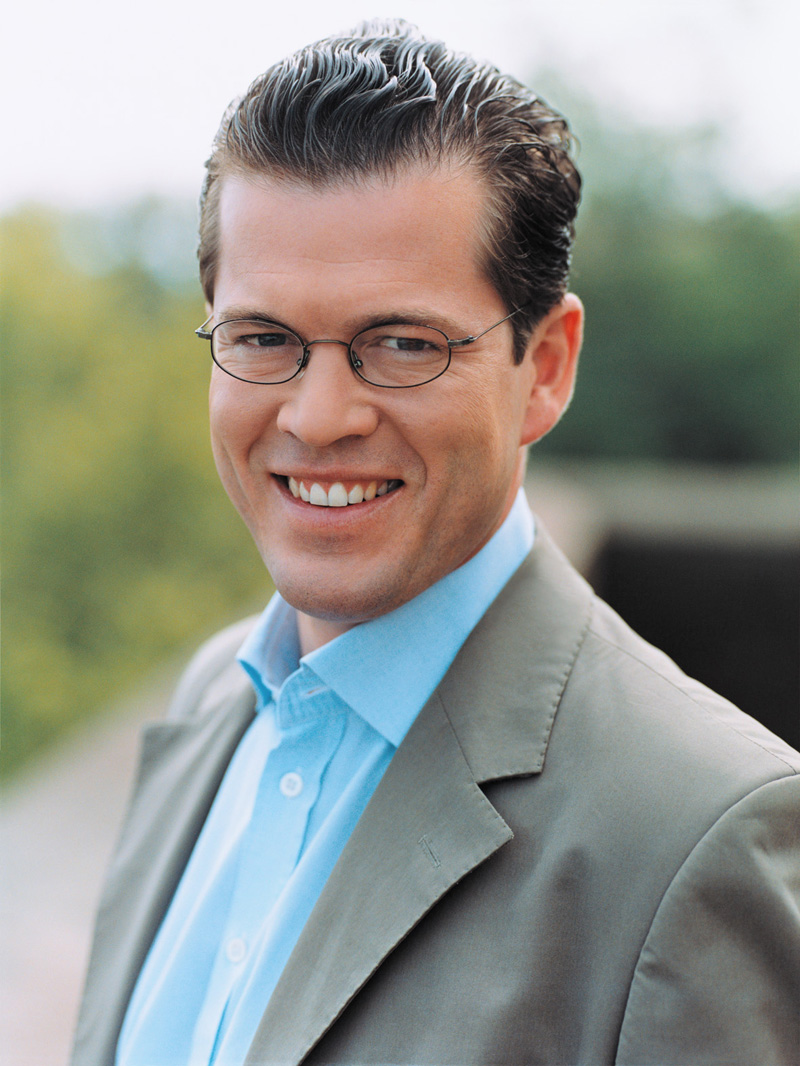
\includegraphics[height=0.85 \textheight]{images/gutti.jpg}
	\end{center}
	
	\textcolor{gray}{\tiny{http://de.wikipedia.org/w/index.php?title=Datei:Guttenberg-800.jpg}}
\end{frame}

\begin{frame}
	\frametitle{Aufgabe 1}		
		\begin{itemize}
			\item Allgemein: Vorsicht bei Beweistechnik
			\begin{itemize}
				\item Ein Gegenbeispiel genügt, um eine Behauptung zu widerlegen.
				\item Ein funktionierendes Beispiel genügt aber \emph{nicht}, um eine Behauptung zu beweisen!
			\end{itemize}
			
			\pause			
			
			\item b) Sei $A$ ein regulärer Ausdruck. Zeige: $(A^*)^* = A^*$
			\begin{itemize}
				\item ''$\supseteq$``: Viele haben argumentiert: $ A \subseteq A^* \Rightarrow A^* \subseteq (A^*)^* $
				\item Die Gleichung $A \subseteq B \Rightarrow A^* \subseteq B^*$ stimmt (warum?), aber muss bewiesen werden!
			\end{itemize}
			
			\pause			
			
			\item d) Seien $A, B, C$ reguläre Ausdrücke. Zeige: $(A \cup B) C = AC \cup BC$ 
			\begin{itemize}
				\item ''Es gilt das Distributivgesetz'' ist keine ausreichende Antwort (genau das soll ja bewiesen werden).
			\end{itemize}
		\end{itemize}
	
\end{frame}
\begin{frame}
	
	\frametitle{Aufgabe 2}
		b) Zeige: Die Schnittmenge zweier regulärer Sprachen ist regulär.
		
		\begin{itemize}
			\item De Morgan'sche Gesetze: $A \cap B = (A^c \cup B^c)^c$ 
			\item Die regulären Sprachen sind unter Vereinigung abgeschlossen (VL).
			\item Es muss aber bewiesen werden: Die regulären Sprachen sind unter Komplementbildung abgeschlossen!
		\end{itemize}
\end{frame}

\begin{frame}
	\frametitle{Aufgabe 3}
		Bestimmen Sie \textbf{nach der Methode aus der Vorlesung} einen regulären Ausdruck für die vom folgenden Automaten erkannte Sprache.
	
		\begin{itemize}
			\item Wenn die Methode aus der Vorlesung gefordert ist, diese bitte auch anwenden.
			\begin{itemize}
				\item Ich weiß, dass das viel Schreibarbeit ist.
				\item Dafür gibt es auch 4 Punkte ;-)
				\item Macht eurem Tutor das Leben leichter				
				\item War schon mal in der Klausur dran (2. Klausur WS 2004/2005)
			\end{itemize}
		\end{itemize}

	
\end{frame}
\begin{frame}
	
	\frametitle{Aufgabe 4}
		Eliminierung von $\varepsilon$-Übergängen $\neq$ Potenzmengenkonstruktion
		\begin{itemize}
			\item Eliminierung von $\varepsilon$-Übergängen: Nur Übergangsfunktion und Endzustandsmenge werden geändert. \\ Resultat: NEA ohne $\varepsilon$-Übergänge
			\item Potenzmengenkonstruktion: Neue Zustände werden eingefügt. \\ Resultat: DEA
		\end{itemize}
\end{frame}

\begin{frame}
	\frametitle{Aufgabe 5}
		\begin{itemize}
		
		\item Haben alle richtig gemacht!
		\item Eventuell mit überflüssigen Zuständen
		\item Verbesserte Methode:
		
		\end{itemize}

	\begin{minipage}{0.3 \textwidth}
		\vspace{0.4cm}
        \begin{tabular}{l|l|l}
		  & 0 & 1 \\
		\hline
		 $s$ & $\{s,q_1\}$ & $\{s\}$ \\
		 $q_1$ 	&	 $\{q_2,f_1\}$	&	$\{f_2\}$  \\
		 $q_2$	&	$\{s,q_2\}$	&	$\{f_2\}$\\
		 $\mathbf{f_1}$ & $\emptyset$ &  $\emptyset$ \\
		 $\mathbf{f_2}$ & $\emptyset$ & $\emptyset$ \\
		\end{tabular}
	
	\end{minipage}
	\setbeamercovered{invisible}
	\pause \hfill
    \begin{minipage}{0.6 \textwidth}        
        \begin{tabular}{l|l|l}
		  & 0 & 1 \\
		\hline
		 $\{s\}$ & \alert<3>{$\{s,q_1\}$} & $\{s\}$ \pause \pause \\
		 \alert<4>{$\{s,q_1\}$} &	 \alert<5>{$\{s,q_1,q_2,f_1\}$}	&	\alert<7>{$\{s,f_2\}$} \pause \pause \\
		 \alert<6>{$\mathbf{\{s,q_1,q_2,f_1\}}$}	&	$\{s,q_1,q_2,f_1\}$	&	$\{s,f_2\}$ \pause \pause \\
		 \alert<8>{$\mathbf{\{s,f_2\}}$}  & $\{s,q_1\}$ &  $\{s\}$ \pause\\
		\end{tabular}
    \end{minipage}		
	
	\hfill
	
	\setbeamercovered{transparent}
\end{frame}

\begin{frame}
	\frametitle{Aufgabe 6}
		\begin{itemize}
			\item Haben auch fast alle richtig!
			\item Bei Aufgabe 6b): $$L=\menge{w\in\{0,1\}^*}{{w \text{ enthält ein Teilwort der Form } 0u0} \atop { \text{ und } \abs{u} \text{ ist durch 4 teilbar}}}$$ \\ Das Teilwort $u$ kann an beliebiger Stelle im Wort vorkommen \\ $\Rightarrow$ Start- und Endzustand haben Übergang zu sich selbst.
		\end{itemize}
\end{frame}

\begin{frame}
	\frametitle{Aufgabe 7}
	
	\begin{itemize}
		\item Gut: Passende Gegenbeispiel-Wörter haben alle gefunden
		\item Weniger gut: Formulierung des Beweises
	\end{itemize}
	
	\pause
	
	\vspace{0,75cm}
	
	Wiederholung: Nicht-Regularitätsbeweis mithilfe des Pumping Lemmas:
	
	\begin{itemize}
		\item Sei $n \in \N$ beliebig, aber fest.
		\item Wähle $w=\text{\textbf{ passendes Wort } mit } w\in L, \abs{w} > n$
		\item Es gilt aber für \textbf{alle} Zerlegungen $w=uvx$ mit $\abs{uv} < n, v\neq \varepsilon$: $uv^\mathbf{42}x \not\in L$, da $\hdots$
		\begin{itemize}
			\item 42 steht hier für eine passend gewählte Zahl $i$, sodass $uv^ix \not\in L$
			\item Manchmal muss $i$ je nach Zerlegung unterschiedlich gewählt werden \\ (auf dem Übungsblatt allerdings nicht).
		\end{itemize}
	\end{itemize}
\end{frame}

\frame{
  \frametitle{Lizenzen}
  \center
  
\includegraphics[width=2em]{images/by}
  
\includegraphics[width=2em]{images/cc}
  
\includegraphics[width=2em]{images/sa}
  \\
  {\tiny

Dieses Werk ist unter einem ``Creative Commons Namensnennung-Weitergabe unter gleichen Bedingungen 3.0 Deutschland``-Lizenzvertrag lizenziert. Um eine Kopie der Lizenz zu erhalten, gehen Sie bitte zu \href{http://creativecommons.org/licenses/by-sa/3.0/de/}{http://creativecommons.org/licenses/by-sa/3.0/de/} oder schreiben Sie an Creative Commons, 171 Second Street, Suite 300, San Francisco, California 94105, USA.\\
  \vspace{1cm}
  Davon ausgenommen sind das Titelbild, welches aus der März-April 2002 Ausgabe von American Scientist erschienen ist und ohne Erlaubnis verwendet wird, sowie das KIT Beamer Theme. Hierfür gelten die Bestimmungen der jeweiligen Urheber.
  \vspace{1cm}
  \\ 
  }
  %Habe hier die Reihenfolge etwas umgestellt, weil die Formatierung bei mir komisch aussah. 
  %Wenn es bei dir anders ist, kannst du es auch wieder zurückändern, dann haben wir unterschiedliche Kompilieroptionen
}

\end{document}
